\chapter{Верификация и примеры расчетов}
\label{sec:verification}

\section{Статическая задача о раскрытие трещины}
\label{sec:static-fracture}
Для верификации алгоритма численного построения матрицы упругости для слоистой среды с неоднородностью модулей упругости была рассмотрена задача о равновесии трещины под действием приложенных нагрузок. Для этого рассматривается круглая трещина и на ее поверхности задается условие постоянного приложенного давления $p$. 

На рисунке~\ref{fig:peirce-2layer} изображено раскрытие круглой трещины, центр которой находится на границе между двумя слоями $y=0$. Коэффициент неоднородности модулей Юнга в слоях $\eta = \frac{E_2}{E_1} = 1$ и 4. Раскрытие трещины нормировано относительно давления $p$ и модуля $E' = E / (1-\nu^2)$. Используя метод разрывных смещений с численно построенной матрицей упругости, получаем раскрытие трещины (сплошная черная линия), которое полностью соответствует результатам работы \cite{Peirce2001UniformAA}.

На рисунке~\ref{fig:peirce-thin-layer} рассматривается раскрытие стационарной круглой трещины в среде, с включением тонкого жесткого слоя $\eta=5$. Результаты численного расчета раскрытия трещины, хорошо сопоставляются с результатами, полученными в работе \cite{Peirce2001TheSF} (среднеквадратическое отклонение менее 6\%).

\begin{figure}[htbp]
    \centering
    \begin{subfigure}[t]{0.4\textwidth}
        \centering
        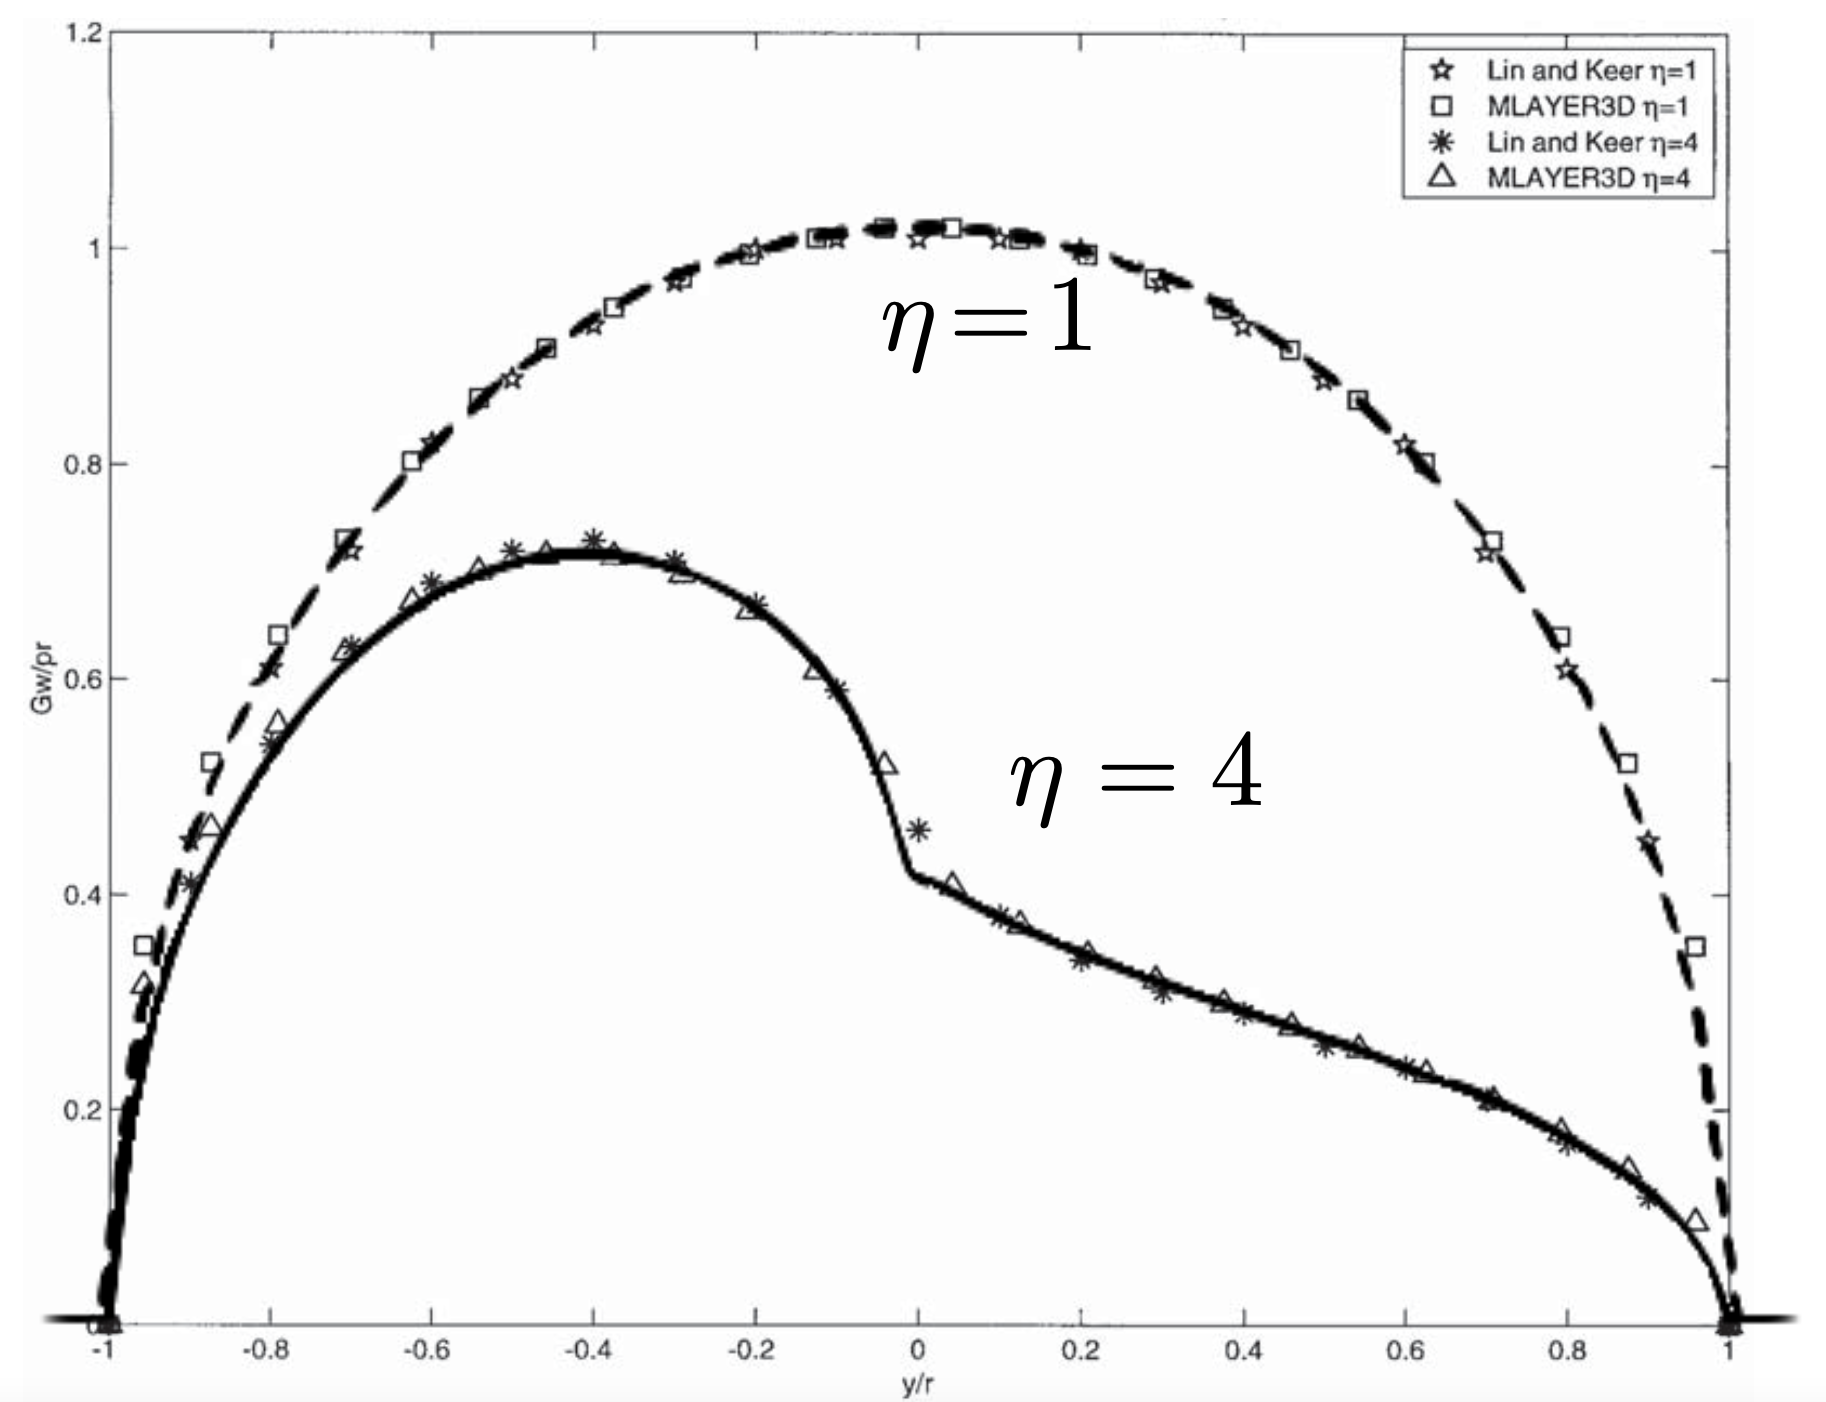
\includegraphics[width=\textwidth]{peirce-2layer.png}
        \caption{Раскрытие трещины, центр которой находится на границе между двумя слоями}
        \label{fig:peirce-2layer}
    \end{subfigure}
    \hfill 
    \begin{subfigure}[t]{0.55\textwidth}
        \centering
        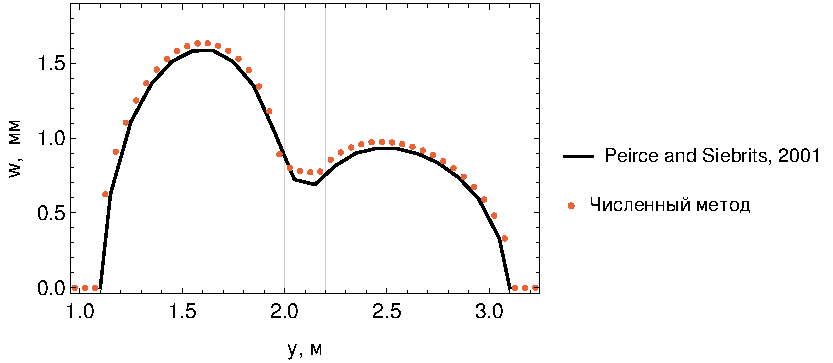
\includegraphics[width=\textwidth]{peirce-thin-layer.pdf}
        \caption{Раскрытие трещины в среде с тонким слоем}
        \label{fig:peirce-thin-layer}
    \end{subfigure}
    \caption{Сравнение результатов расчета с оцифрованными данными из работ \cite{Peirce2001UniformAA,Peirce2001TheSF}}
    \label{fig:comparison-peirce}
\end{figure}


\section{Задача о раскрытие трещины ГРП}
Рассмотрим модель распространения трещины ГРП с равномерной по времени закачкой объема жидкости из скважины. Начальный момент времени $t = 0$~c, конечный $t = 300$~с, утечки жидкости ГРП, связанные с ее фильтрацией из трещины в пласт, отсутствуют. Для демонстрации влияния неоднородности модулей упругости рассмотрим пласт, состоящий из трех слоев. Точка закачки жидкости ГРП находится в центре внутреннего слоя. Толщина внутреннего слоя равна $20$ м. $E_i$, $\nu_i$, где $i=\text{b, m, t}$ --- упругие модули нижнего, среднего и верхнего слоев соответственно. $\sigma_{h,i}$, где $i=\text{b, m, t}$ --- сжимающие напряжения. В силу симметрии среды и ее параметров в горизонтальном направление расчет раскрытия трещины ГРП проводится только для одной половины.

\subsection{Неоднородность модулей упругости}
В случае, если упругие модули всех слоев одинаковы получается модель радиальной трещины (рисунки \ref{fig:homogeneous-planar}, \ref{fig:homogeneous-slice}).
\begin{figure}[htbp]
    \centering
    \begin{subfigure}[t]{0.4\textwidth}
        \centering
        \includegraphics[width=\textwidth]{Homogeneous/Figures/1/width_29.pdf}
        \caption{Раскрытие трещины.}
        \label{fig:homogeneous-planar}
    \end{subfigure}
    \hfill 
    \begin{subfigure}[t]{0.55\textwidth}
        \centering
        \includegraphics[width=\textwidth]{Homogeneous/Figures/1/w_y_29.pdf}
        \caption{Раскрытие трещины вдоль оси $Oy$, $x=1.5$~м.}
        \label{fig:homogeneous-slice}
    \end{subfigure}
    \caption{Радиальная трещина, $E_\text{b} = E_\text{m} = E_\text{t} = 10$~GPa, $\nu_\text{b} = \nu_\text{m} = \nu_\text{t} = 0.22$.}
    \label{fig:homogeneous}
\end{figure}

Рассмотрим пласт, где модуль Юнга $E_\text{b}$ нижнего слоя выше, чем в верхних. Как видно из рисунков~\ref{fig:heterogeneous-2-layer-planar} и \ref{fig:heterogeneous-2-layer-slice} жесткость нижнего слоя сильно влияет на распространение трещины. Полученная конечная геометрия трещины кардинально отличается от радиальной трещины (рисунок~\ref{fig:homogeneous}). Расстояние от верхнего кончика трещины до точки закачки жидкости ГРП в два раза больше, чем расстояние от нижнего кончика трещины до точки закачки.
\begin{figure}[htbp]
    \centering
    \begin{subfigure}[t]{0.4\textwidth}
        \centering
        \includegraphics[width=\textwidth]{Heterogeneous/Figures/1/width_29.pdf}
        \caption{Раскрытие трещины.}
        \label{fig:heterogeneous-2-layer-planar}
    \end{subfigure}
    \hfill 
    \begin{subfigure}[t]{0.55\textwidth}
        \centering
        \includegraphics[width=\textwidth]{Heterogeneous/Figures/1/w_y_29.pdf}
        \caption{Раскрытие трещины вдоль оси $Oy$, $x=1.5$~м.}
        \label{fig:heterogeneous-2-layer-slice}
    \end{subfigure}
    \caption{Пласт с жестким нижним слоем, $E_\text{b} = 50$~GPa, $E_\text{m} = E_\text{t} = 10$~GPa, $\nu_\text{b} = \nu_\text{m} = \nu_\text{t} = 0.22$.}
    \label{fig:heterogeneous-2-layer}
\end{figure}

Также на распространение трещины ГРП и ее конечную геометрию влияет и неоднородность сжимающих напряжений. Слой с высокой величиной сжимающего напряжения способен образовать барьер, который ограничивает рост трещины в вертикальном направление. Однако, этот эффект не наблюдается при неоднородности по модулям упругости. Даже при большой разнице между упругими модулями в слоях трещина проникает и растет вдоль жесткого слоя. Это подтверждается результатом моделирования роста трещины ГРП, изображенной на рисунке~\ref{fig:heterogeneous-high}, где коэффициент неоднородности $\eta=\frac{E_\text{b}}{E_\text{t}} = 10$. На рисунке~\ref{fig:heterogeneous-3layer} показан случай, где модуль Юнга среднего слоя $E_\text{m}$ в $\eta=10$ раз меньше, чем у ограничивающих его слоев. Однако, помимо роста в горизонтальном направление (вдоль границы между слоями), трещина растет и в вертикальном направление, проникая в жесткие слои. Подобный результат был также продемонстрирован на модели Pseudo3d в работе~\cite{gu2006}.
\begin{figure}[htbp]
    \centering
    \begin{subfigure}[t]{0.4\textwidth}
        \centering
        \includegraphics[width=\textwidth]{Heterogeneous/Figures/2/width_29.pdf}
        \caption{Раскрытие трещины.}
        \label{fig:heterogeneous-high-planar}
    \end{subfigure}
    \hfill 
    \begin{subfigure}[t]{0.55\textwidth}
        \centering
        \includegraphics[width=\textwidth]{Heterogeneous/Figures/2/w_y_29.pdf}
        \caption{Раскрытие трещины вдоль оси $Oy$, $x=1.5$~м.}
        \label{fig:heterogeneous-high-slice}
    \end{subfigure}
    \caption{Пласт с сильной неоднородностью, $E_\text{b} = 100$~GPa, $E_\text{m} = E_\text{t} = 10$~GPa, $\nu_\text{b} = \nu_\text{m} = \nu_\text{t} = 0.22$}
    \label{fig:heterogeneous-high}
\end{figure}


\begin{figure}[htbp]
    \centering
    \begin{subfigure}[t]{0.4\textwidth}
        \centering
        \includegraphics[width=\textwidth]{Heterogeneous/Figures/3_3/width_29.pdf}
        \caption{Раскрытие трещины.}
        \label{fig:heterogeneous-3layer-planar}
    \end{subfigure}
    \hfill 
    \begin{subfigure}[t]{0.55\textwidth}
        \centering
        \includegraphics[width=\textwidth]{Heterogeneous/Figures/3_3/w_y_29.pdf}
        \caption{Раскрытие трещины вдоль оси $Oy$, $x=1.5$~м.}
        \label{fig:heterogeneous-3layer-slice}
    \end{subfigure}
    \caption{Пласт с сильной неоднородностью, $E_\text{m} = 10$~GPa, $E_\text{b} = E_\text{t} = 100$~GPa, $\nu_\text{b} = \nu_\text{m} = \nu_\text{t} = 0.22$}
    \label{fig:heterogeneous-3layer}
\end{figure}


\subsection{Неоднородность модулей упругости и сжимающих напряжений}
Рассмотрим пласт, где присутствует одновременно неоднородность сжимающих напряжений и модулей упругости в слоях. В верхних слоях $\sigma_{h,\text{m}} = \sigma_{h,\text{t}} = 30.5$~MPa выше, чем в нижнем $\sigma_{h,\text{b}} = 30$~MPa. Из рисунка~\ref{fig:comparison-1} видно, что рост трещины ГРП обусловлен ростом в нижнем слое, несмотря на то, что его модуль Юнга $E_\text{b} = 20$~GPa больше, чем в верхних слоях $E_\text{m} = E_\text{t} = 10$~GPa. Подобное поведение распространения трещины связано с тем, что величина эффективного напряжения $p_\text{net} = p - \sigma_h$ --- выше в нижнем слое. Из уравнения~\eqref{eq:elasticity_equation} видно, что эффективное напряжение $p_\text{net}$ напрямую влияет на величину раскрытия трещины. На рисунке~\ref{fig:comparison-2} приведен пример, где модуль Юнга нижнего слоя $E_\text{b} = 40$~GPa компенсирует высокое эффективное напряжение, и рост трещины ГРП происходит как в верхнем, так и нижнем вертикальными направлениями.

\begin{figure}[htbp]
    \centering
    \begin{subfigure}[t]{0.4\textwidth}
        \centering
        \includegraphics[width=\textwidth]{Heterogeneous/Figures/3/width_29.pdf}
        \caption{Раскрытие трещины.}
        \label{fig:comparison-1-planar}
    \end{subfigure}
    \hfill 
    \begin{subfigure}[t]{0.55\textwidth}
        \centering
        \includegraphics[width=\textwidth]{Heterogeneous/Figures/3/w_y_29.pdf}
        \caption{Раскрытие трещины вдоль оси $Oy$, $x=1.5$~м.}
        \label{fig:comparison-1-slice}
    \end{subfigure}
    \caption{Неоднородный по модулям упругости и сжимающим напряжениям пласт, $E_\text{b} = 20$~GPa, $E_\text{m} = E_\text{t} = 10$~GPa, $\nu_\text{b} = \nu_\text{m} = \nu_\text{t} = 0.22$, $\sigma_{h,\text{b}} = 30$~MPa, $\sigma_{h,\text{m}} = \sigma_{h,\text{t}} = 30.5$~MPa.}
    \label{fig:comparison-1}
\end{figure}


\begin{figure}[htbp]
    \centering
    \begin{subfigure}[t]{0.4\textwidth}
        \centering
        \includegraphics[width=\textwidth]{Heterogeneous/Figures/3_2/width_29.pdf}
        \caption{Раскрытие трещины.}
        \label{fig:comparison-2-planar}
    \end{subfigure}
    \hfill 
    \begin{subfigure}[t]{0.55\textwidth}
        \centering
        \includegraphics[width=\textwidth]{Heterogeneous/Figures/3_2/w_y_29.pdf}
        \caption{Раскрытие трещины вдоль оси $Oy$, $x=1.5$~м.}
        \label{fig:comparison-2-slice}
    \end{subfigure}
    \caption{Неоднородный по модулям упругости и сжимающим напряжениям пласт, $E_\text{b} = 40$~GPa, $E_\text{m} = E_\text{t} = 10$~GPa, $\nu_\text{b} = \nu_\text{m} = \nu_\text{t} = 0.22$, $\sigma_{h,\text{b}} = 30$~MPa, $\sigma_{h,\text{m}} = \sigma_{h,\text{t}} = 30.5$~MPa.}
    \label{fig:comparison-2}
\end{figure}


\subsection{Включение тонкого жесткого пропластка в пласт}
Рассмотрим пласт, где присутствует включение тонкого жесткого слоя (толщина слоя $d$ меньше $10\%$ от диаметра трещины). Как видно из рисунков~\ref{fig:thin-layer-1} и \ref{fig:thin-layer-2} тонкие жесткие пропластки не ограничивают рост трещины. Диаметр трещины ГРП в горизонтальном направление практически совпадает с диаметром в вертикальном направление. Однако раскрытие в них ниже, чем в прилегающих слоях. Это может существенно сказаться на распространение проппанта и конечной геометрии трещины ГРП. 
\begin{figure}[htbp]
    \centering
    \begin{subfigure}[t]{0.4\textwidth}
        \centering
        \includegraphics[width=\textwidth]{Heterogeneous/Figures/4/width_29.pdf}
        \caption{Раскрытие трещины.}
    \end{subfigure}
    \hfill 
    \begin{subfigure}[t]{0.55\textwidth}
        \centering
        \includegraphics[width=\textwidth]{Heterogeneous/Figures/4/w_y_29.pdf}
        \caption{Раскрытие трещины вдоль оси $Oy$, $x=1.5$~м.}
    \end{subfigure}
    \caption{Пласт с включением тонкого слоя, $d=10$~м. , $k=\frac{E_d}{E}=5$.}
    \label{fig:thin-layer-1}
\end{figure}

\begin{figure}[htbp]
    \centering
    \begin{subfigure}[t]{0.4\textwidth}
        \centering
        \includegraphics[width=\textwidth]{Heterogeneous/Figures/5/width_29.pdf}
        \caption{Раскрытие трещины.}
    \end{subfigure}
    \hfill 
    \begin{subfigure}[t]{0.55\textwidth}
        \centering
        \includegraphics[width=\textwidth]{Heterogeneous/Figures/5/w_y_29.pdf}
        \caption{Раскрытие трещины вдоль оси $Oy$, $x=1.5$~м.}
    \end{subfigure}
    \caption{Пласт с включением двух тонких пропластков, $d=10$~м. , $k=\frac{E_d}{E}=5$.}
    \label{fig:thin-layer-2}
\end{figure}